% http://latex-cookbook.net/cookbook/examples/releux-triangle/
\documentclass{standalone}
\usepackage{tkz-euclide}
\usetkzobj{all}
\begin{document}
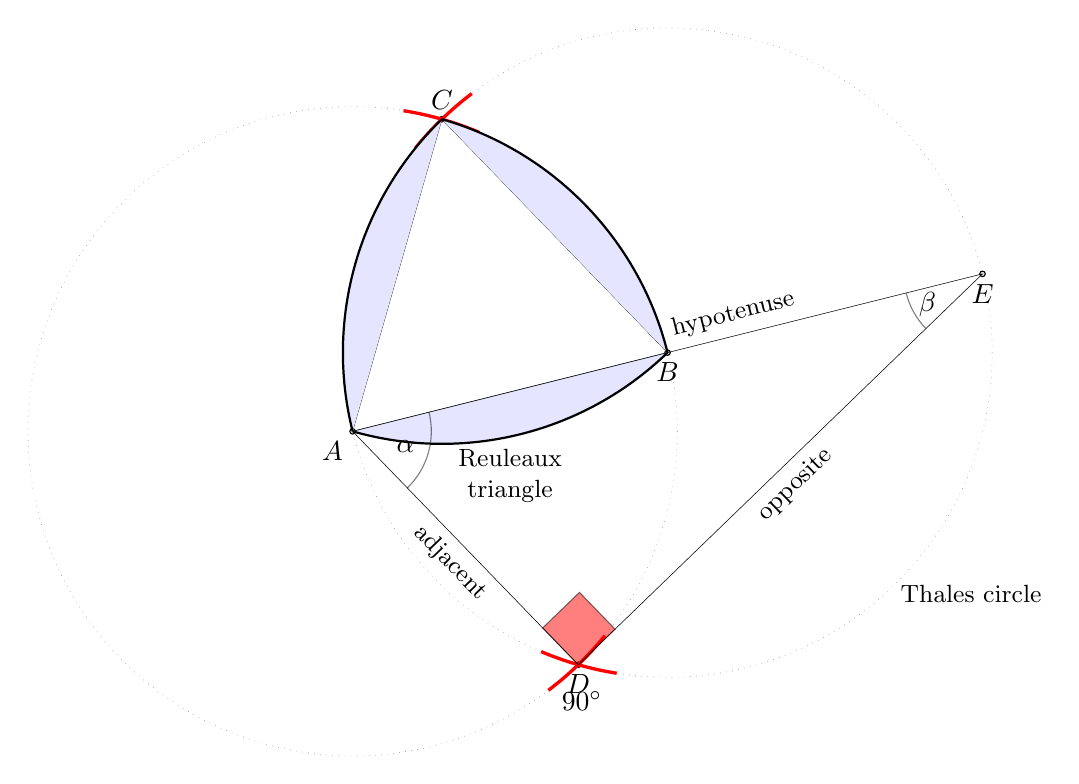
\begin{tikzpicture}
	\tkzDefPoint(0,0){A}
	\tkzDefPoint(4,1){B}
	\tkzInterCC(A,B)(B,A)
	\tkzGetPoints{C}{D}
	
	\tkzDrawPolygon(A,B,C)
	\tkzDrawPoints(A,B,C,D)
	
	\tkzLabelPoints[below left](A)
	\tkzLabelPoints(B,D)
	\tkzLabelPoint[above](C){$C$}
	
	\tkzDrawCircle[dotted](A,B)
	\tkzDrawCircle[dotted](B,A)
	
	\tkzCompass[color=red, very thick](A,C)
	\tkzCompass[color=red, very thick](B,C)
	
	\tkzCompass[color=red, very thick](A,D)
	\tkzCompass[color=red, very thick](B,D)
	
	\tkzDrawArc[fill=blue!10,thick](A,B)(C)
	\tkzDrawArc[fill=blue!10,thick](B,C)(A)
	\tkzDrawArc[fill=blue!10,thick](C,A)(B)
	
	\tkzInterLC(A,B)(B,A)
	\tkzGetPoints{F}{E}
	\tkzDrawPoints(E)
	\tkzLabelPoints(E)
	\tkzDrawPolygon(A,E,D)
	
	\tkzMarkAngles[fill=yellow,opacity=0.5](D,A,E A,E,D)
	\tkzMarkRightAngle[size=0.65,fill=red,opacity=0.5](A,D,E)
	\tkzLabelAngle[pos=0.7](D,A,E){$\alpha$}
	\tkzLabelAngle[pos=0.8](A,E,D){$\beta$}
	\tkzLabelAngle[pos=0.5,xshift=-1.4mm](A,D,D){$90^\circ$}
	
	\tkzLabelSegment[below=0.6cm,align=center,font=\small](A,B){Reuleaux\\triangle}
	\tkzLabelSegment[above right,sloped,font=\small](A,E){hypotenuse}
	\tkzLabelSegment[below,sloped,font=\small](D,E){opposite}
	\tkzLabelSegment[below,sloped,font=\small](A,D){adjacent}
	\tkzLabelSegment[below right=4cm,font=\small](A,E){Thales circle}
\end{tikzpicture}
\end{document}